\def\bookfile{mother_of_hydrogen.pdf}
\def\booktitle{Mother of Hydrogen}

% Paper weight used
\input{papers}
\def\bookpaper{\lxxxgsm}


\newcounter{bookpagecount}
\setcounter{bookpagecount}{\XeTeXpdfpagecount"\bookfile"}
\RequirePackage{calc} % This line must be after the previous to avoid an error
\newlength{\outsidepaperwidth} % no. of pages ÷ 2 × width per sheet
\setlength{\outsidepaperwidth}{\bookpaper * \value{bookpagecount} / \real{2.0}}

\newlength{\outsidespinewidth} % paper thickness
\setlength{\outsidespinewidth}{\outsidepaperwidth}
\makeatletter
\setbox\z@=\hbox{\XeTeXpdffile"\bookfile"\relax}
\newlength{\outsidecoverwidth} % paper width
\setlength{\outsidecoverwidth}{\the\wd\z@}
\newlength{\outsidecoverheight} % coverheight: paper height
\setlength{\outsidecoverheight}{\the\ht\z@}
\makeatother
\documentclass[12pt,coverwidth=\the\outsidecoverwidth,coverheight=\the\outsidecoverheight,spinewidth=\the\outsidespinewidth,marklength=0mm,bleedwidth=5mm]{bookcover}

\usepackage{contour}
\usepackage{moh}

% N.B. All text and images should be 6mm away from all edges
\begin{document}
\begin{bookcover}
    \bookcovercomponent{normal}{bg whole}{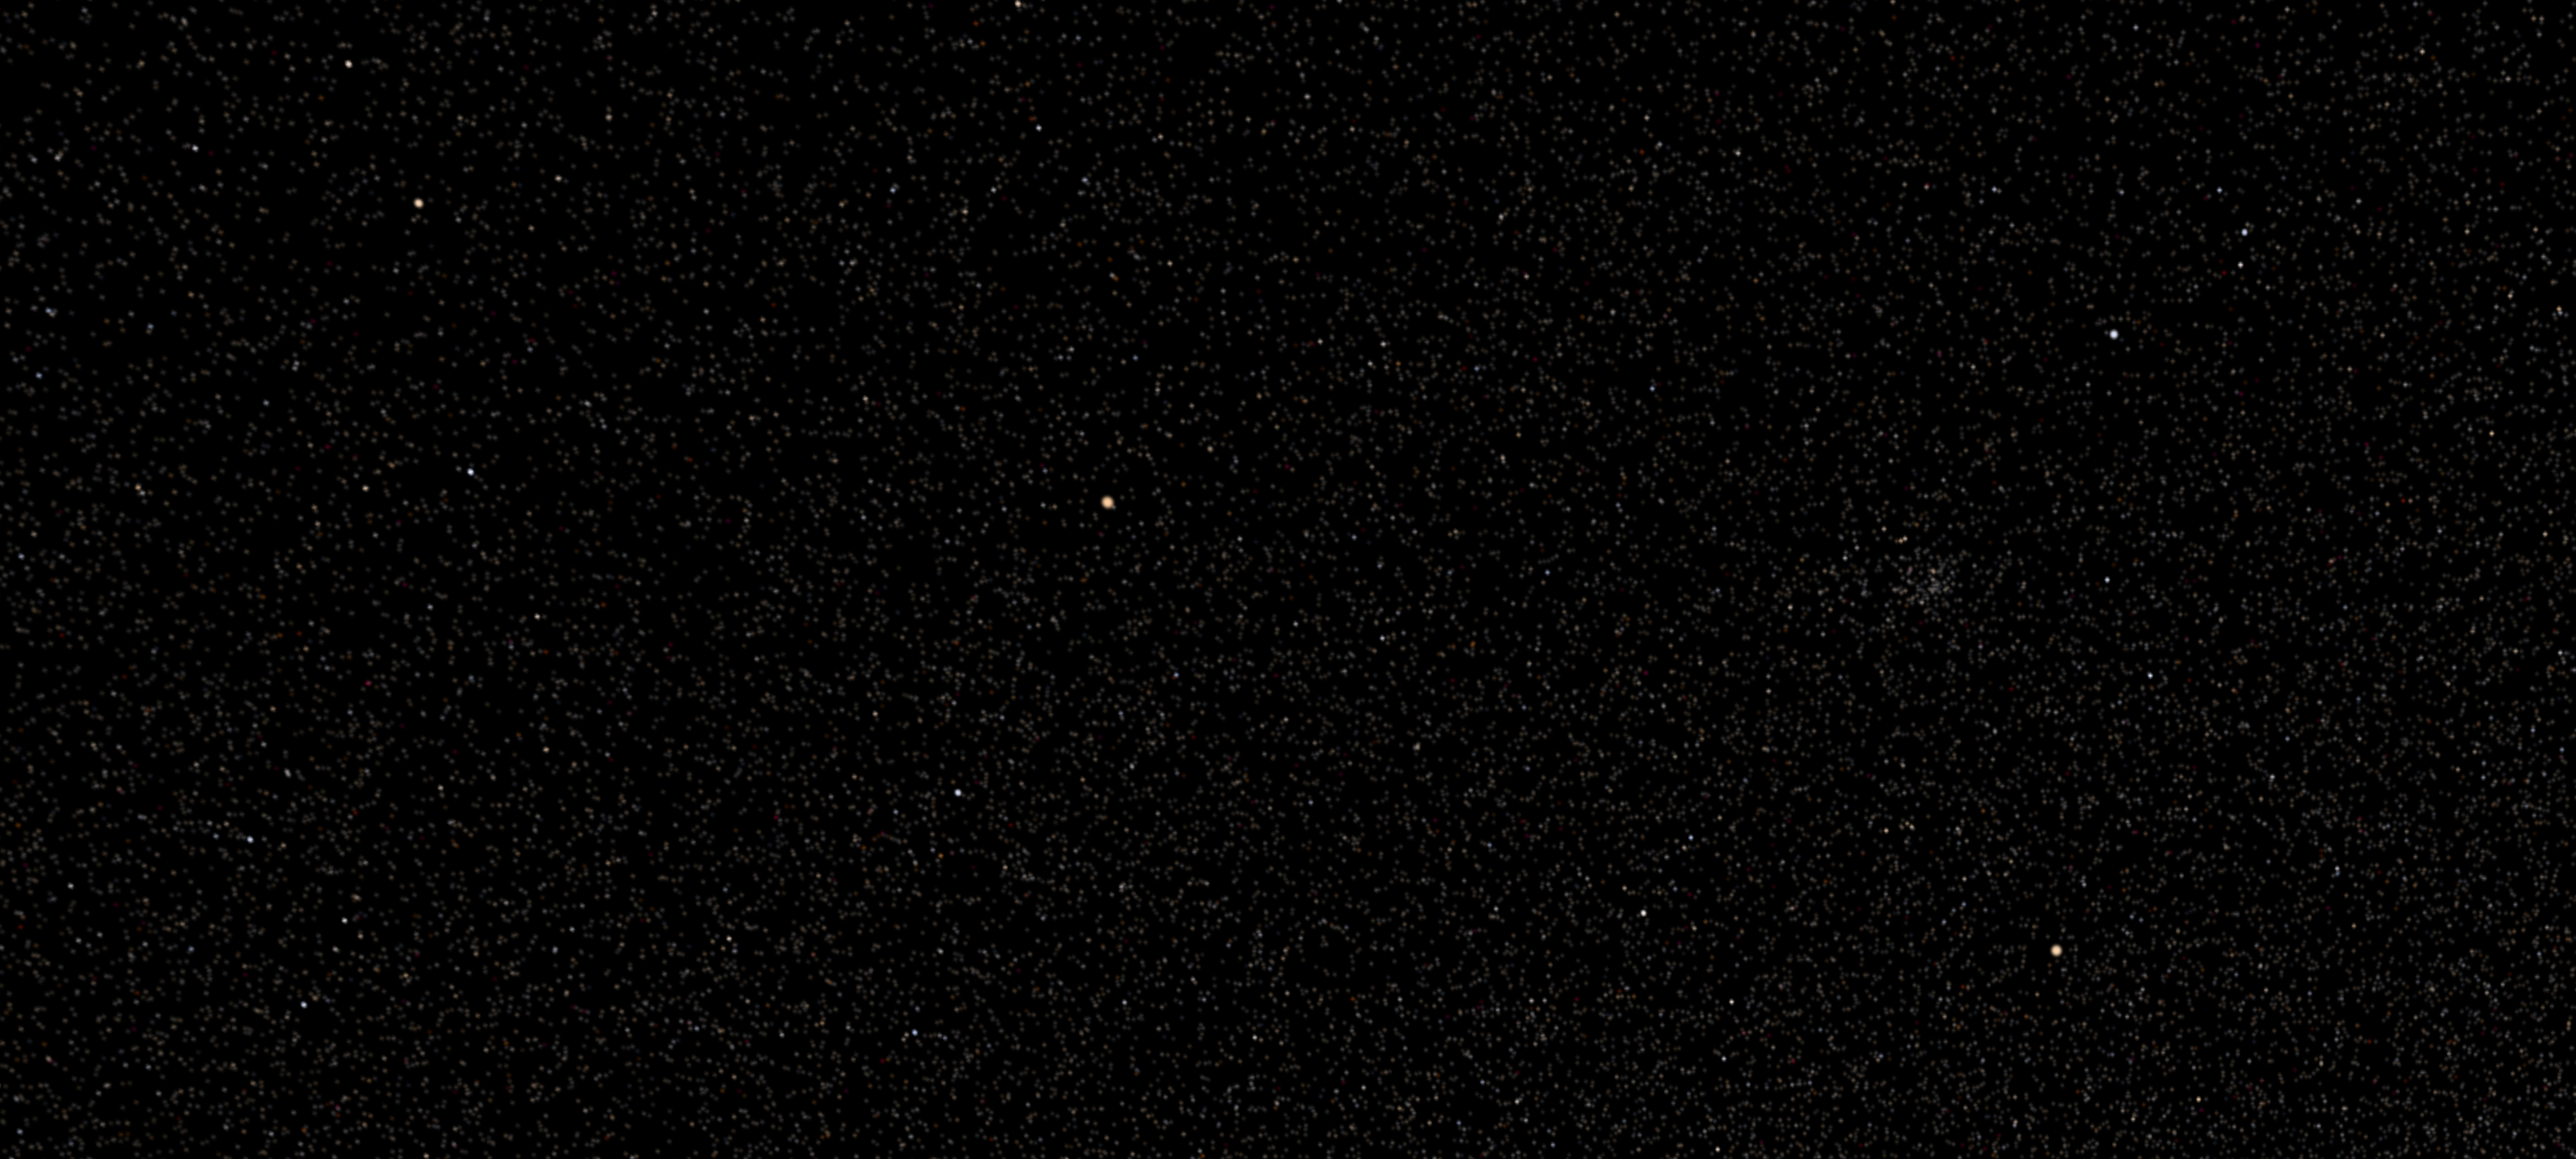
\includegraphics[width=550mm]{background.jpg}} % TODO: Why not 520mm, which is correct for aspect ratio?

  %\bookcovercomponent{normal}{front}{\color{white}\begin{center}\vspace{2cm}\bf{\Huge Mother of Hydrogen}\\[2cm]{\LARGE The Future We Deserve}\\[10cm]{\LARGE A Novel}\\[2cm]{\Huge Vinay Gupta}\\[2cm]{\Large Hexayurt Press}\end{center}}
  \bookcovercomponent{picture}{front}{Cover-transparent.png}

  \bookcovercomponent{center}{spine}{%
    \color{white}\LARGE\rotatebox[origin=c]{90}{\contour[120]{black}{\booktitle}}}

  \bookcovercomponent{normal}{back}{%
    \centering%
    \vspace{20mm}%
    \parbox{110mm}{\color{white}\Large\raggedright
      In the second half of the twenty-first century, a resurgent America dominates the world with its global humanitarian–military mission. Fifteen-year-old Harry Vine is about to start his mandatory national service. His father Gregory has reservations despite a career spent as a drone-jockey, and his uncle Peter, a hippie drop-out, is determined to prevent his joining the new brainwashed generation.

      Meanwhile in space, where all the really interesting tech is quarantined, an infant AI has become convinced it is the only conscious being in the known universe…
    }}

\end{bookcover}
\end{document}

% Local Variables:
% ispell-local-dictionary: "american"
% End:
